% Este arquivo .tex será incluído no arquivo .tex principal. Não é preciso
% declarar nenhum cabeçalho

\section{Diversão}
\subsection{Espaços culturais}


\begin{itemize}
\item  \textbf{Casa do Lago:} Dentro da Unicamp, mantém uma programação quase diária de cinema e exposições. Este ano estão viabilizando a instalação de café e revistaria. A página da casa do lago é: \url{www.preac.rei.unicamp.brcasadolago/}.
\end{itemize}

\begin{itemize}
\item  \textbf{Semente:} Fica no fim da avenida Santa Isabel, depois da moradia. Sempre tem apresentações artísticas, como teatros e espetáculos musicais.
\end{itemize}

\subsection{Cinemas}

\begin{itemize}
\item  \textbf{Kinoplex (15 salas).}
\begin{itemize}
\item  Endereço: Shopping D. Pedro (Rodovia Dom Pedro I, Km 137 -- Jd. Sta. Genebra).
\item  Telefone: (19) 3131-2800.
\item  Site: \url{www.kinoplex.com.br}
\end{itemize}
\end{itemize}

\begin{itemize}
\item  \textbf{Cinemark Iguatemi (8 salas).}
\begin{itemize}
\item  Endereço: Shopping Center Iguatemi (Avenida Iguatemi, 777 -- Vila Brandina).
\item  Telefone: (19) 3251-1122.
\item  Site: \url{www.cinemark.com.br}
\end{itemize}
\end{itemize}

\begin{itemize}
\item  \textbf{Cine Jaraguá (2 salas).}
\begin{itemize}
\item  Endereço: Shopping Prado (Bairro Parque Prado).
\item  Telefone: (19) 3243-6537.
\item  Site: \url{www.cinejaragua.com.br}
\end{itemize}
\end{itemize}

\begin{itemize}
\item  \textbf{Box Cinemas (10 salas).}
\begin{itemize}
\item  Endereço: Campinas Shopping (Rua Jacy T. de Camargo, 940 -- Jardim do Lago).
\item  Telefone: (19) 4003-7097.
\item  Site: \url{www.boxcinemas.com.br}
\end{itemize}
\end{itemize}

\begin{itemize}
\item  \textbf{Cine Galleria (7 salas).}
\begin{itemize}
\item  Endereço: Galleria Shopping (Rod. Dom Pedro I, Km, 131,5 -- Jd. Nilópolis).
\item  Telefones: (19) 3207-0982.
\item  Site: \url{www.galleria.com.br/page/cinema.asp}
\end{itemize}
\end{itemize}

\begin{itemize}
\item  \textbf{Cine Moviecom Unimart (4 salas).}
\begin{itemize}
\item  Endereço: Shopping Unimart (Avenida John Boyd Dunlop, 350 -- Chácara da República).
\item  Telefone: (19) 3243-5206.
\item  Site: \url{www.moviecom.com.br/index.php?id=CAM}
\end{itemize}
\end{itemize}

\begin{itemize}
\item  \textbf{Sala Cine Paradiso.}
\begin{itemize}
\item  Endereço: Galeria Barão Velha (Rua Barão de Jaguara, 936 -- Centro).
\item  Telefone: (19) 3234-4741.
\end{itemize}
\end{itemize}

\begin{itemize}
\item  \textbf{Cine Evolução/MIS (1 sala)}
\begin{itemize}
\item  Endereço: Rua Regente Feijó, 1087 -- Centro
\item  Telefone: (19) 3232-9959
\end{itemize}
\end{itemize}

\subsection{Teatros}

\begin{itemize}
\item  \textbf{Lume Teatro}
    \begin{itemize}
        \item  Endereço:  Rua Carlos Diniz Leitão, 150 Vila Santa Isabel -- Barão Geraldo
        \item  Telefone: (19) 3289-9869
        \item  Site: \url{www.lumeteatro.com.br}
    \end{itemize}

\item  \textbf{Teatro Interno Luiz Otávio Burnier}
    \begin{itemize}
        \item  Endereço: Centro de Convivência Cultural (Praça Imprensa Fluminense s/nº -- Cambuí)
        \item  Telefone: (19) 3252-5977
    \end{itemize}

\item  \textbf{Teatro de Arena}
    \begin{itemize}
        \item  Endereço: Centro de Convivência Cultural (Praça Imprensa Fluminense s/nº -- Cambuí)
        \item  Telefone: (19) 3252-5977
    \end{itemize}

\item  \textbf{Teatro Carlos Maia}
    \begin{itemize}
        \item  Endereço: Rua Cel. Quirino, 2 -- Bosque dos Jequitibás
        \item  Telefone: (19) 3231-8795
    \end{itemize}

\item  \textbf{Teatro José de Castro Mendes}
    \begin{itemize}
        \item  Endereço: Praça Corrêa de Lemos, s/nº -- Vila Industrial
        \item  Telefone: (19) 3272-9359
    \end{itemize}

\item  \textbf{Auditório Beethoven (Concha Acústica)}
    \begin{itemize}
        \item  Endereço: Avenida Heitor Penteado, s/nº -- Portão 2 -- Lagoa do Taquaral
        \item  Telefone: (19) 3256-9959
    \end{itemize}

\item  \textbf{Teatro de Arte e Ofício}
    \begin{itemize}
        \item  Endereço: Rua Conselheiro Antônio Prado, 529 -- Vila Nova
        \item  Telefone: (19) 3241-7217
    \end{itemize}

\item  \textbf{Teatro Dom Nery (Externato São João)}
    \begin{itemize}
        \item  Endereço: Rua José de Alencar, 360  Centro
        \item  Telefone: (19) 3231-2644
    \end{itemize}

\item  \textbf{Teatro Teresa Aguiar (Conservatório)}
    \begin{itemize}
        \item  Endereço: Rua José de Alencar, 701 -- Centro
        \item  Telefone: (19) 3232-9345
    \end{itemize}

\item  \textbf{Teatro da Vila Padre Anchieta}
    \begin{itemize}
        \item  Endereço: Avenida Cardeal Dom Agnelo Rossi, s/nº -- Vila Padre Anchieta
        \item  Telefone: (19) 3781-0382
    \end{itemize}

\item  \textbf{Centro Cultural Evolução}
    \begin{itemize}
        \item  Endereço: Rua Regente Feijó, 1087 -- Centro
        \item  Telefone: (19) 3232-9959
    \end{itemize}

\item  \textbf{Teatro TIM}
    \begin{itemize}
        \item  Endereço: Shopping D. Pedro, Entrada das flores
        \item  Telefones: (19) 3756-9890 e (19) 3756-9891
    \end{itemize}

\end{itemize}

\subsection{Boates e baladas}

\begin{figure}[hb!]
    \centering
    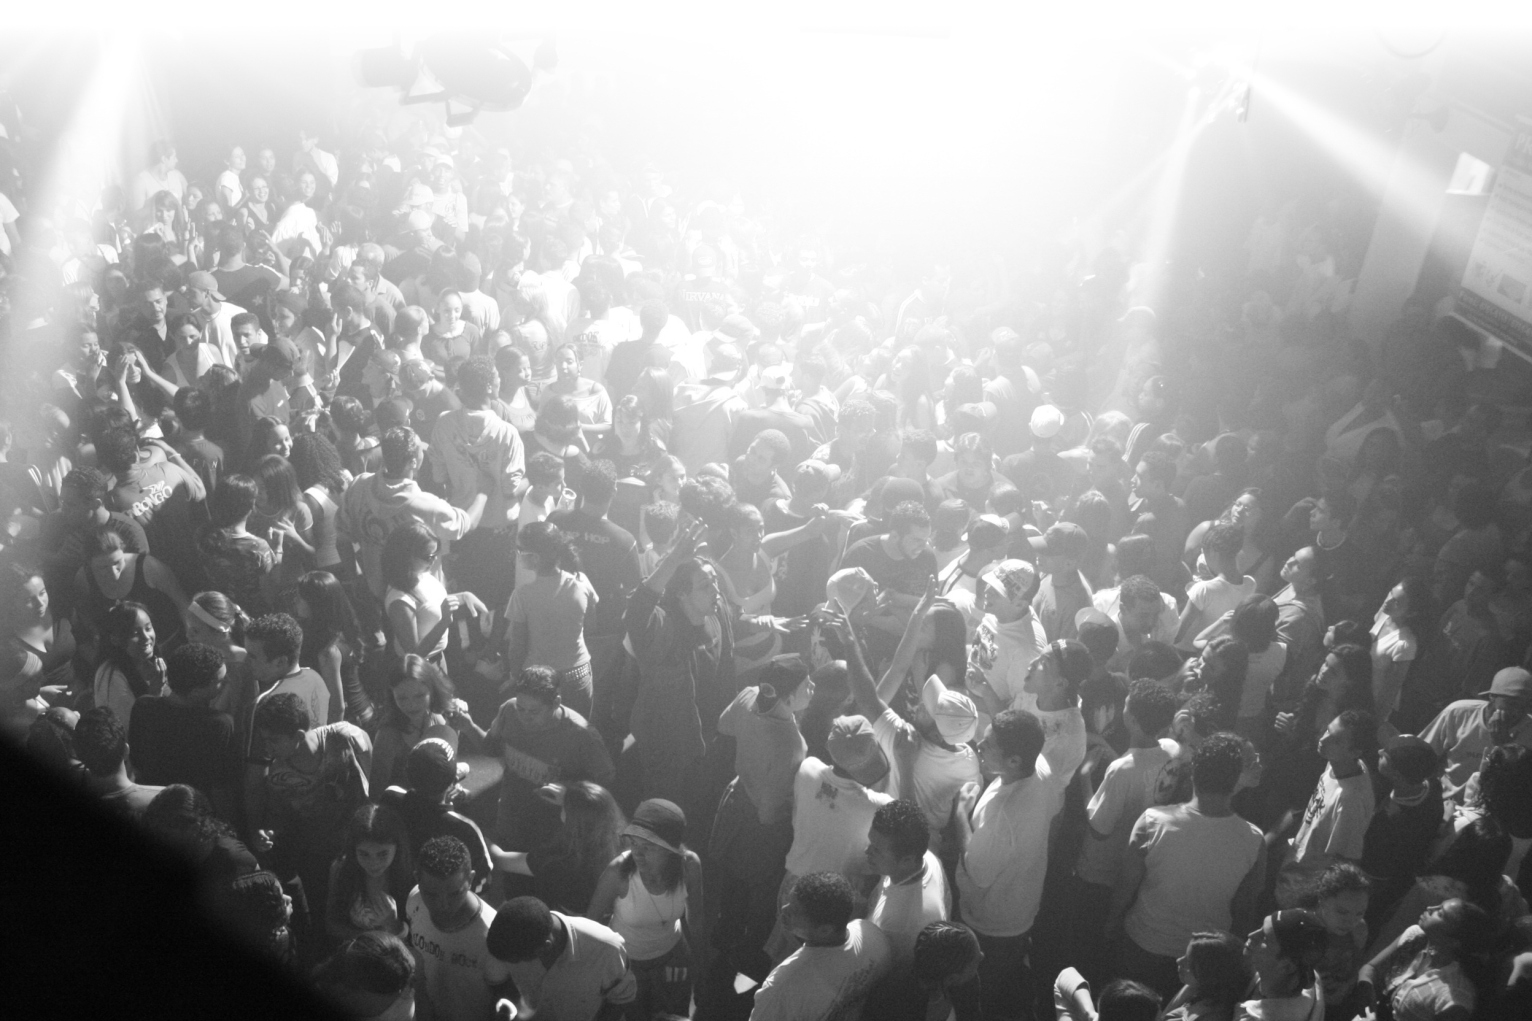
\includegraphics[scale=0.15,keepaspectratio=true]{img/imgs/7-diversao/-053.jpg}
\end{figure}

\begin{itemize}
\item  \textbf{Cooperativa Brasil:} Para quem gosta de um bom forró, sempre com
    shows diversos. A galera gosta muito da quarta-universitária. Maiores
    informações, acesse o site: \url{www.cooperativabrasil.com.br}.

\item  \textbf{Campinas Hall:} Muitas das festas mais legais da Unicamp
    acontecem lá (como a Festa Brega e a Festa do Contrário), perto da PUCC.
    É bem grande.

\item  \textbf{Delta Blues Bar:} O melhor do Blues \& Rock 'n Roll de Campinas
    \url{www.deltabluesbar.com.br}.

\item  \textbf{Barril da Máfia:} \url{www.barrildamafia.com.br}.

\item  \textbf{Swingers:} Tem bebidas caras e cada noite tem um tema, mas
    é melhor às quartas e quintas-feiras. Só homens maiores de 21 e mulheres com
    mais de 18 anos podem entrar.
    \url{www.grupohappynews.com.br/novo/swingers_campinas/index.php}

\item  \textbf{Golden:} Assim como a Swingers fica no Shopping D. Pedro. Balada
    cara, frequentada geralmente por gente mais velha.
    \url{www.goldstreetbar.com.br}

\item  \textbf{Camaleão Show:} Antigo Club Diesel. Primeira casa noturna de
    micareta e pagode de Campinas. \url{www.camaleaoshow.com.br}

\item  \textbf{Kraft:} Localizada próxima ao Taquaral (na Avenida Imperatriz
    Leopoldina), toca musica psi a noite toda e fica aberta até quase
    o amanhecer. Mulher entra de graça até a meia-noite.
    \url{www.clubekraft.com/}

\item  \textbf{Cambuí:} Neste bairro existem diversos barzinhos, a maioria
    é temático, alguns são um pouco caros e cobram covert. É um ótima escolha
    para quem tiver carro pois fica um pouco longe de Barão.

\end{itemize}

\subsection{Shopping Centers}

\begin{figure}[h!]
    \centering
    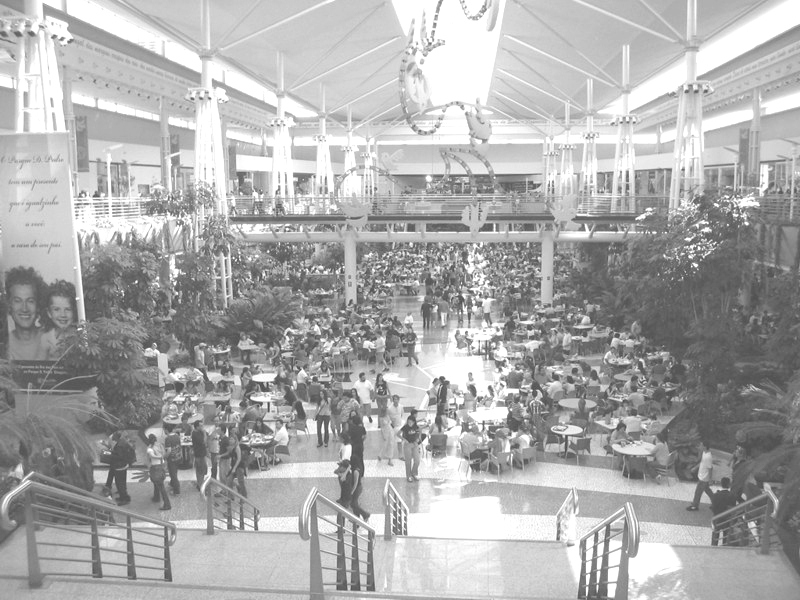
\includegraphics[scale=0.28,keepaspectratio=true]{img/imgs/7-diversao/-057.jpg}
\end{figure}

\begin{itemize}

\item  \textbf{Shopping Parque D. Pedro:} Foi considerado o maior shopping da
    América Latina até pouco tempo atrás. Localiza-se na Rodovia Dom Pedro, km
    137 (razoavelmente próximo a Unicamp). O ônibus 3.38 sai do terminal Barão
    vai para lá e para o Iguatemi. Outras opções de ônibus saindo do terminal
    são 2.10 e 3.00. Página do shopping:
    \url{www.parquedpedro.com.br}.

\item  \textbf{Shopping Iguatemi:} Shopping normal, o mais antigo e o segundo
    maior de Campinas. Localiza-se na Avenida Iguatemi, 777. O 3.38 demora uns
    40 minutos para chegar lá. Frequentado pela galera mais nova e pelo pessoal
    com um pouco mais de dinheiro. Página do shopping:
    \url{www.iguatemicampinas.com.br}.

\item  \textbf{Shopping Jaraguá:} Shopping pequeno e que possui duas unidades:
    Uma delas fica na Rua Conceiçao (Jaraguá Conceição); e a outra unidade fica
    na avenida Brasil (Jaraguá Brasil). Nesse segundo há duas salas de cinema
    que passam filmes "cult". O ônibus 3.30, no sentido terminal central --
    Unicamp para razoavelmente próximo ao Jaraguá Conceição, um ponto antes do
    ponto da prefeitura; e os ônibus 3.30, 3.31, 3.32 e 3.33 passam em frente ao
    Jaraguá Brasil.

\item  \textbf{Campinas Shopping:} Longe a dar com pau, mas as lojas não são
    muito caras. Localiza-se às margens das rodovias Anhanguera e Santos Dumont.
    Provavelmente você nunca irá lá. Página do shopping:
    \url{www.campinasshopping.com.br}.

\item  \textbf{Shopping Prado:} Shopping bem pequeno, as lojas não são muito
    caras, mas muito longe. Localiza-se na Avenida Washington Luís, 2480.
    Provavelmente você também nunca irá lá.

\item  \textbf{Galleria Shopping:} Muito bonito, mas lojas muito caras. Também
    localizado na Rodovia Dom Pedro, mas no km 131,5. O ônibus 3.00 sai do
    terminal de Barão Geraldo e passa lá. Página do shopping:
    \url{www.galleria.com.br}.

\item  \textbf{Shopping Unimart:} Shopping pequeno, as lojas não são muito
    caras. Localiza-se na Avenida John Boyd Dunlop, 350. O ônibus 1.34 sai do
    terminal de Barão Geraldo e passa próximo. Página do shopping:
    \url{www.unimart.com.br}.

\end{itemize}
